%課題研究レジュメテンプレート ver. 1.0

\documentclass[uplatex]{jsarticle}
\usepackage[top=20mm,bottom=20mm,left=20mm,right=20mm]{geometry}
\usepackage[T1]{fontenc}
\usepackage{txfonts}
\usepackage{wrapfig}
\usepackage[expert,deluxe]{otf}
\usepackage[dvipdfmx,hiresbb]{graphicx}

\makeatletter
  \renewcommand{\section}{%
    \if@slide\clearpage\fi
    \@startsection{section}{1}{\z@}%
    {\Cvs \@plus.5\Cdp \@minus.2\Cdp}% 前アキ
    {.5\Cvs \@plus.3\Cdp}% 後アキ
    %{\normalfont\Large\headfont\raggedright}}
    {\normalfont\raggedright}}

  \renewcommand{\subsection}{\@startsection{subsection}{2}{\z@}%
    {\Cvs \@plus.5\Cdp \@minus.2\Cdp}% 前アキ
    {.5\Cvs \@plus.3\Cdp}% 後アキ
    %{\normalfont\large\headfont}}
    {\normalfont}}

  \renewcommand{\subsubsection}{\@startsection{subsubsection}{3}{\z@}%
    {\Cvs \@plus.5\Cdp \@minus.2\Cdp}%
    {\z@}%
    %{\normalfont\normalsize\headfont}}
    {\normalfont}}
\makeatother
%ここから上を編集する必要はない.





\title{\vspace{-14mm}クラウドファンディングにおける成功の判別分析}
\author{PMコース 矢吹研究室 1242105 三浦泰介}
\date{}%日付を入れる必要はない.
\pagestyle{empty}%ページ番号は振らない.
\begin{document}
\maketitle





\section{研究の背景}
世界中の様々なところでクラウドファンディングを利用したプロジェクトが行われており,日本においてもクラウドファンディングで資金集めを行ったプロジェクトを多く聞くようになっている.
クラウドファンディングとはプロジェクトの必要資金を,インターネットを利用し,不特定多数の支援者から資金提供を募集する資金調達の手法である.大手企業から個人のプロジェクトまで幅広い規模のプロジェクトで応募が可能であり,近年ベンチャー企業や学生にチャンスを与えるものとして注目を集めている.クラウドファンディングは一般的に資金提供者に対するリターンの形態によって以下の3つに分けることができる.
\begin{enumerate}
 \item 金銭的リターンのない「寄付型」
 \item 金銭的リターンのある「投資型」
 \item 権利や物品を購入することで支援する「購入型」
\end{enumerate}

日本では金融商品取引法が2014年に改正されるまで法規制の問題から,見返りを得ない寄付に近いものか,購入型に限られていたため購入型が主流になっている.\cite{wiki} \cite{keizai}今回,日本でプロジェクトを起こすことを考え,大手クラウドファンディングサイトであるCAMPFIRE\cite{campfire}とMakuake\cite{makuake}に掲載されているプロジェクトから,購入型のプロジェクトの成功要因を探すことにする.




\section{研究の目的}

CAMPFIREとMakuake掲載されているプロジェクトから支援の金額,コースの数など支援者側から見える情報をデータとして集め,決定木を描くことでクラウドファンディングにおける成功要因を明らかにすることを目指す.







\section{プロジェクトマネジメントとの関連}

クラウドファンディングの成功要因を明らかにすることで,資金集めの段階でのプロジェクト成功確率を上げることができると考えられる.






\section{研究の方法}

以下の手順で研究を行った.
\begin{enumerate}
 \item CAMPFIREとMakuakeのプロジェクトの中から監視するプロジェクトを選定する.
 \item 定期的にプロジェクトのウェブページを保存することでプロジェクトの進捗を監視する.
 \item プロジェクトの設定や支援者から知り得る情報を元に判別分析を行う,
 \item 決定木を書き,プロジェクトの成功要因を考察し,成功合否の判別を行う.
\end{enumerate}

\section{現在の進捗状況}
\subsection{結果}
集めたデータから要因を抽出し,決定木を作成したところ決定木図1が得られた.決定木作成に使用したデータを表1として掲載クラウドファンディングではプロジェクトごとに決められたコースが用意されている.支援者はコースの支援金額に応じた商品や権利を支援の報酬として手に入れることができる。その支援コースの数が7.5以上で成功率が86\%,支援コースの数が7.5以下の場合では成功率が28\%という結果が得られた.また支援コースの数が7.5以下の中でも支援コースの数が3.5以上の場合,成功率が67\%と支援コースの数が3.5以下で20\%と成功率の差が47\%出るという結果も出ている.
\subsection{考察}
クラウドファンディングにおいて支援コースの数が成功に大きく関わっている事がわかった.支援コースの数が8項目以上の場合,成功率が86\%支援コースの数が4以上の場合,成功率が67\%.支援コースの数が4以下で成功率に20\%と言う結果から,クラウドファンディングを行う際には支援コースの数が8項目以上設定することが好ましく,8項目が無理でも4項目以上設定しなければ成功率が著しく低くなってしまうことが言える。


\makeatletter
\def\setcaption#1{\def\@captype{#1}}
\makeatother

\begin{center}

\begin{minipage}{10cm}
  \setcaption{figure}
\caption{決定木作成で使用したデータ}\label{サンプル図}
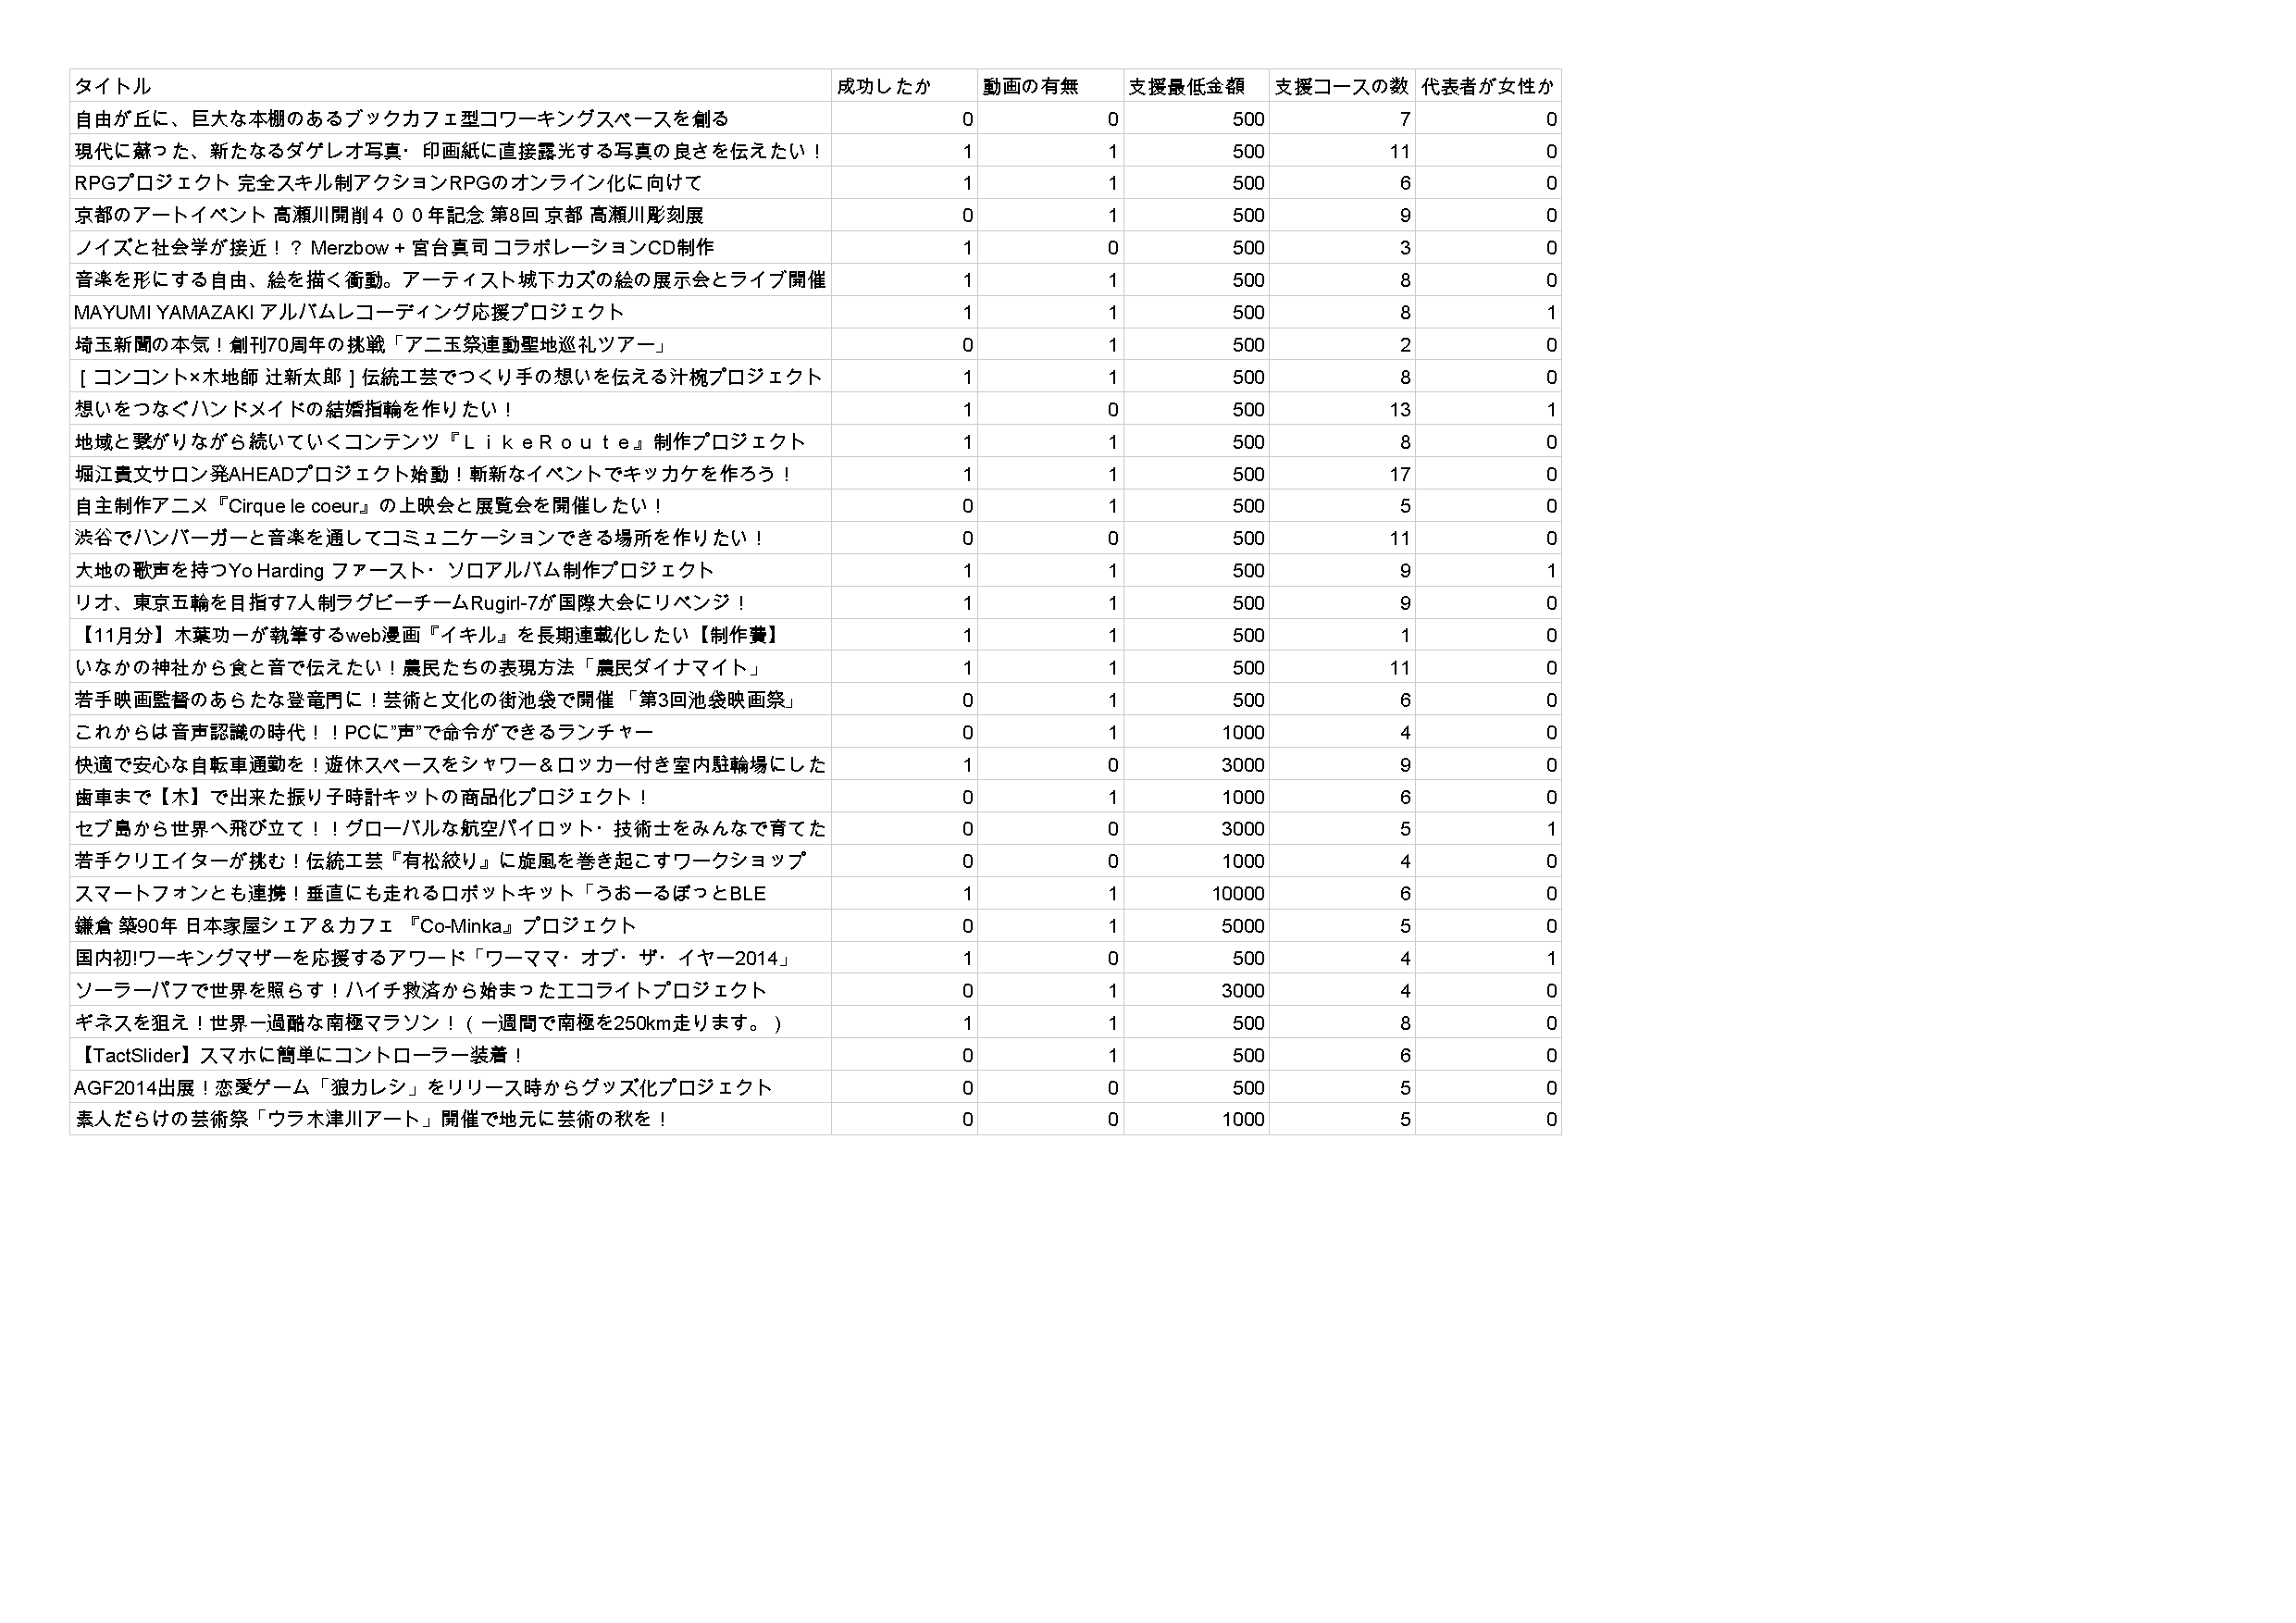
\includegraphics[width=10cm,clip]{figure2.pdf}
\end{minipage}
\begin{minipage}{6cm}
  \setcaption{table}
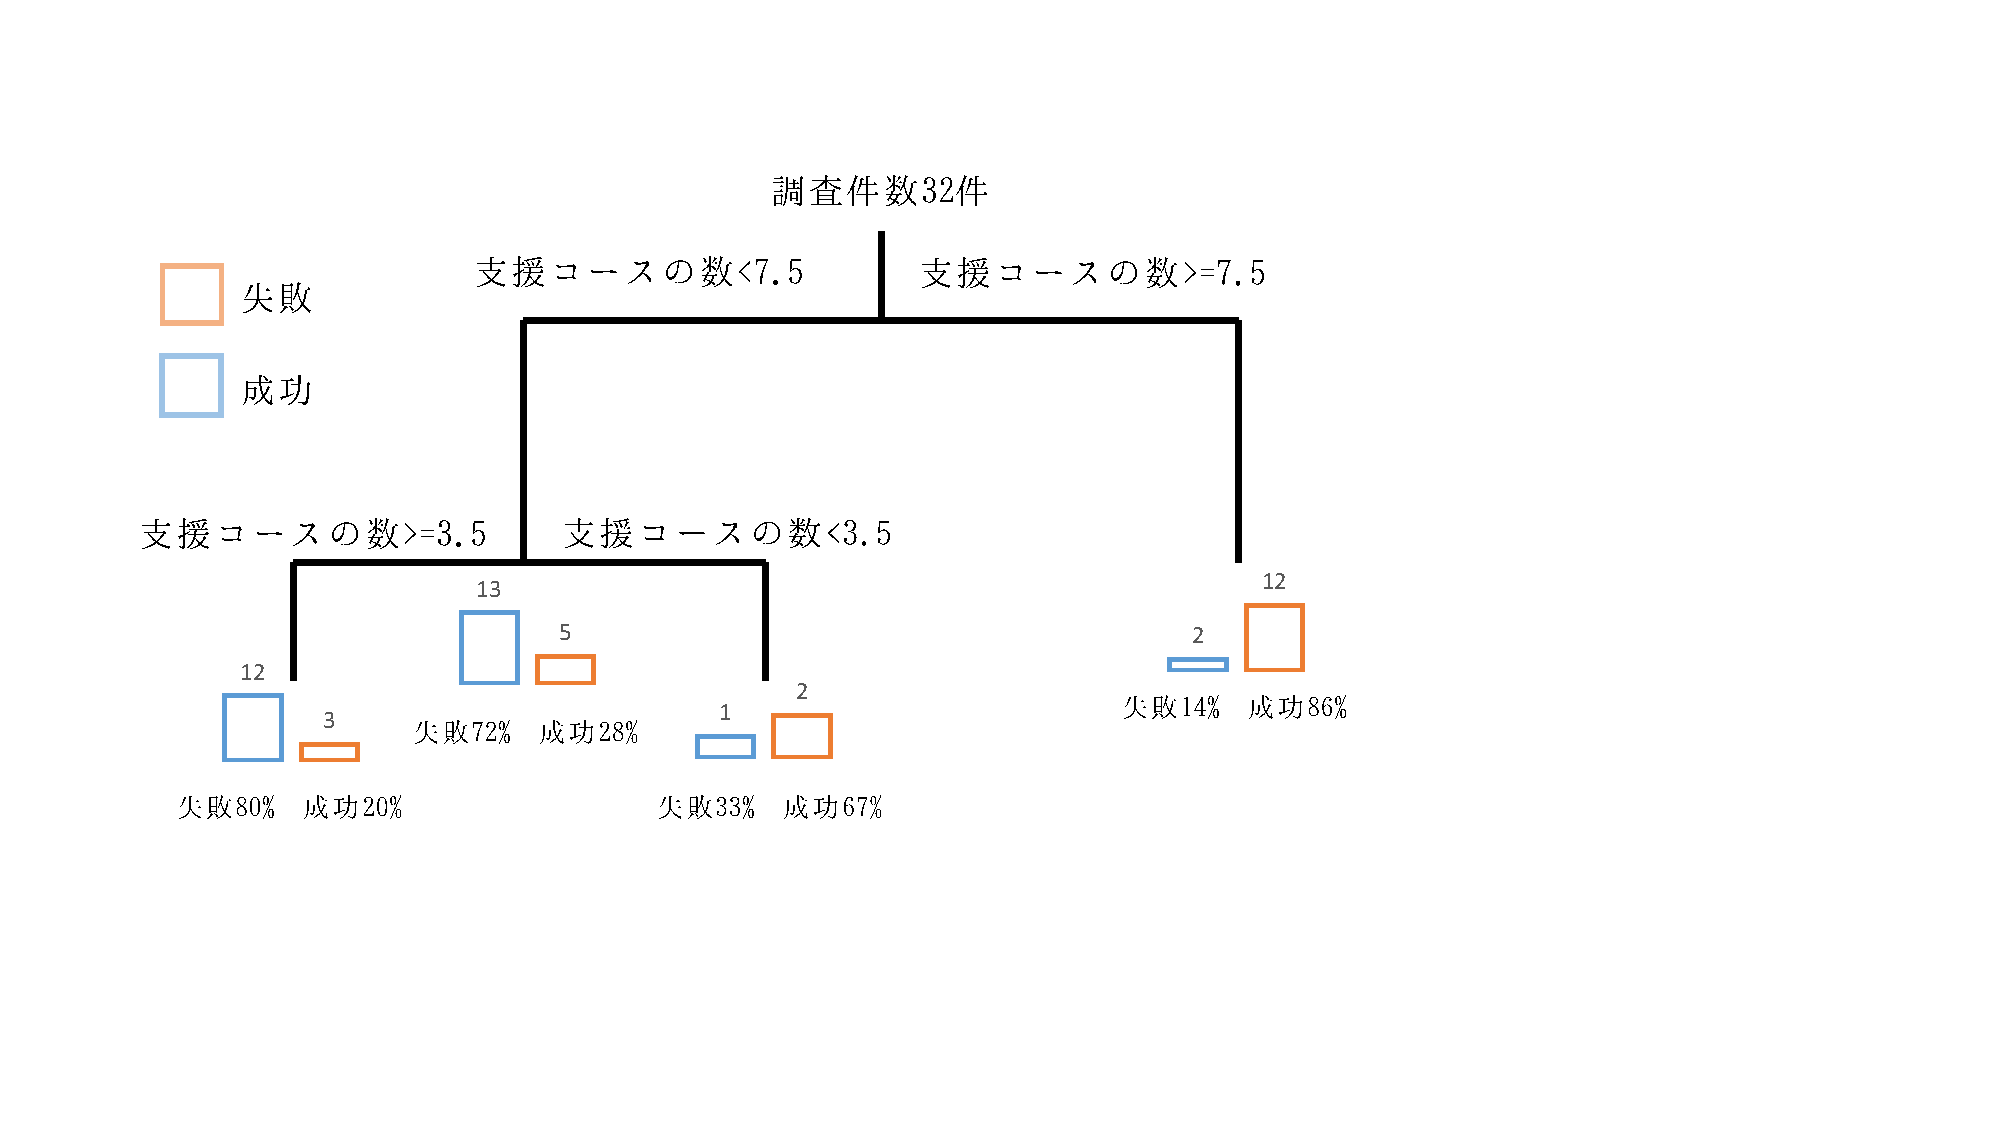
\includegraphics[width=6cm,clip]{figure.pdf}
 \caption{決定木作成で使用したデータ}\label{サンプル図}  
\end{minipage}
\end{center}


\section{今後の計画}
今後、更に多くのプロジェクトを監視し,多くのデータを用いて解析を行うことで,今回の結果の信憑性をあげるとともに、他にも成功に大きく関わる要因を見つけ出す事を目標とする.
以下のように研究を進める計画である.

\begin{enumerate}
\item データを自動で集められるように環境を整える.
\item 監視するクラウドファンディングのサイトを増やしデータ数を増やす.
\item 解析を行う要因を増やす.判別分析を行い成功に関わりが強い要因を調査する.
\item 判別分析の結果から,始まったばかりのプロジェクトの成功合否を予測し,どの程度実際の成功と一致しているかを確かめる.
\end{enumerate}


\bibliographystyle{junsrt}
\bibliography{biblio}%「biblio.bib」というファイルが必要.

\end{document}